% !TEX program = xelatex

\documentclass{ctexart}
\usepackage{ctex}
\usepackage[a4paper, left=20mm, right=20mm, top=30mm, bottom=30mm]{geometry}
\usepackage{graphicx}
\graphicspath{ {./images/} }
\usepackage{amsmath}
\usepackage{hyperref}
\hypersetup{
  colorlinks=true,
  linkcolor=black
}
\usepackage{xcolor}
\usepackage{listings}

% listings宏包配置,引用自:
% 怎么在 LaTeX 中排版 Python 代码? - 孟晨的回答 - 知乎
% https://www.zhihu.com/question/65508676/answer/232267619
\lstdefinestyle{lfonts}{
  basicstyle   = \footnotesize\ttfamily,
  stringstyle  = \color{purple},
  keywordstyle = \color{blue!60!black}\bfseries,
  commentstyle = \color{olive}\scshape,
}
\lstdefinestyle{lnumbers}{
  numbers     = left,
  numberstyle = \tiny,
  numbersep   = 1em,
  firstnumber = 1,
  stepnumber  = 1,
}
\lstdefinestyle{llayout}{
  breaklines       = true,
  tabsize          = 2,
  columns          = flexible,
}
\lstdefinestyle{lgeometry}{
  xleftmargin      = 20pt,
  xrightmargin     = 0pt,
  frame            = tb,
  framesep         = \fboxsep,
  framexleftmargin = 20pt,
}
\lstdefinestyle{lgeneral}{
  style = lfonts,
  style = lnumbers,
  style = llayout,
  style = lgeometry,
}
\lstdefinestyle{python}{
    language = {Python},
    style    = lgeneral,
}

\author{
	冯国蕴 \and 林欣煜 \and 马詠汛 \and 谢金宏
}
\title{使用细胞自动机模拟简单生态系统}
\date{2019年12月21日}

\begin{document}

\maketitle

\begin{abstract}
在本次课题中,我们小组使用Python语言实现了基本的细胞自动机。并在已有的细胞自动机的规则基础上进行扩展,尝试对具有氧气、生产者和消费者三要素的生态系统进行模拟,并将模拟的结果以图像形式表示。
\end{abstract}

\tableofcontents

\newpage

\listoffigures

\newpage

\section{细胞自动机与康威生命游戏}

细胞自动机\footnote{Cellular automaton \url{https://en.wikipedia.org/wiki/Cellular_automaton}}最早由冯·诺依曼在1950年代为模拟生物细胞的自我复制而提出,起初未受到科学界的广泛关注。其后约翰·何顿·康威设计了生命游戏\footnote{Conway's Game of Life \url{https://en.wikipedia.org/wiki/Conway's_Game_of_Life}}而让细胞自动机闻名于世。本节将简要介绍细胞自动机与康威生命游戏。

\subsection{细胞自动机}

我们可以在二维的格状棋盘上实现一个细胞自动机。在这个二维的空间上,棋盘中每个格子内细胞的状态是有限的,细胞下一时刻的状态由该细胞的邻居在当前的时刻的状态决定。棋盘内的所有细胞遵守相同的演化规则。

一个细胞自动机一般具有以下特点:

\begin{itemize}
  \item \textbf{平行计算 }每个细胞个体的状态都同步地进行改变。
  \item \textbf{局部性 }细胞的状态只受相邻的细胞的影响。
  \item \textbf{一致性 }所有的细胞受到相同的规则约束。
\end{itemize}

\subsection{康威生命游戏}

康威生命游戏在细胞自动机的基础上,定义了细胞演化的规则:

\begin{itemize}
  \item 每种细胞有“存活”和“死亡”两种状态。
  \item 当细胞周围的存活细胞数量等于3个时,细胞变为存活状态。
  \item 当细胞周围的存活细胞数量少于等于1个或大于等于4个时,细胞变为死亡状态。(模拟细胞过于孤独或环境过于拥挤。)
  \item 其他情况下细胞状态不变。
\end{itemize}

我们小组使用Python实现了经典的康威生命游戏(\underline{1.basic.py})。程序先随机地给定棋盘内细胞初始状态,然后按照康威生命游戏规则演化指定的代数,给出最终的结果。

\begin{figure}[ht]
  \centering
  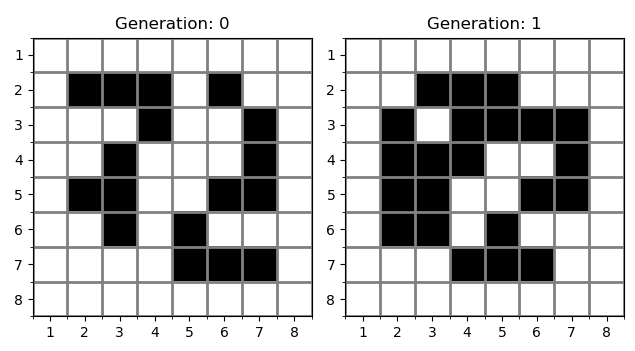
\includegraphics[scale=0.75]{cellular-automation.png}
  \caption{按康威生命游戏规则进行一次迭代}
  \label{fig:cellular-automation}
\end{figure}

图\ref{fig:cellular-automation}是随机产生初始状态后按康威规则演化一代的结果。图中黑色块表示活细胞,白色块表示没有活细胞的空位。

\subsection{镜像边界}

细胞自动机理论上具有无穷大的“棋盘”作为细胞演化的空间,但计算机的内存空间是有限的,故无限大的棋盘不能实现,实际运行中的棋盘往往是边长为$n$的矩形棋盘。有限的空间就存在边界问题,需要特殊处理边界上的细胞。

在\underline{1.basic.py}中,边界上的细胞不参与演化,它们总是保持死细胞的状态。这是处理边界问题的一种方法,即边界上的细胞总是取定值,在演化过程中保持不变。

另一种处理边界细胞问题的方法是在\underline{1.basic-mirror-edge.py}中实现的镜像边界方法。如图\ref{fig:mirror-edge-example}所示,编号为1的细胞,它的左上角邻居、左邻居和右邻居分别被镜像地设置为9号、3号和7号细胞。

\begin{figure}[ht]
  \centering
  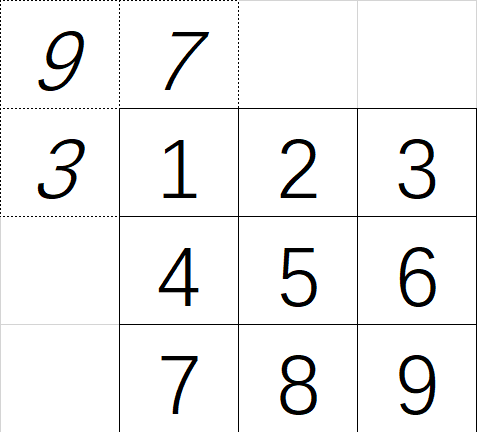
\includegraphics[scale=0.6]{mirror-edge-example.png}
  \caption{镜像边界的一个实例}
  \label{fig:mirror-edge-example}
\end{figure}

一般地,对于采用镜像边界的$SIZE$大小的棋盘,格点位置为$(i, j)$的细胞,它的邻居可以通过如下程序遍历:

\begin{lstlisting}[style = python]
for i, j in CELLS:
  for dx in range(-1, 2):
    for dy in range(-1, 2):
      neighbor = board.iat[(i + dx + SIZE) % SIZE, (j + dy + SIZE) % SIZE]
\end{lstlisting}

如无特殊说明,本文后续的模型均采用镜像边界的处理方法。

\subsection{康威生命游戏的几个经典图案}

我们在程序中实现了康威生命游戏的几个经典图形。这些图形中,有一些永远保持“静止”,不发生变化(如图\ref{fig:classic-fixed});有一些则是周而复始的图形(如图\ref{fig:classic-vibrating})。

\begin{figure}[ht]
  \centering
  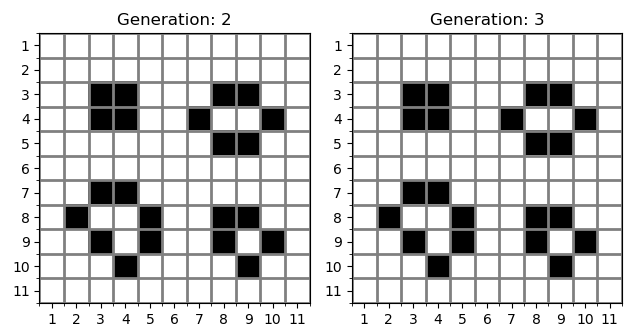
\includegraphics[scale=0.75]{classic-fixed.png}
  \caption{永远保持静止的图形}
  \label{fig:classic-fixed}
\end{figure}

\begin{figure}[ht]
  \centering
  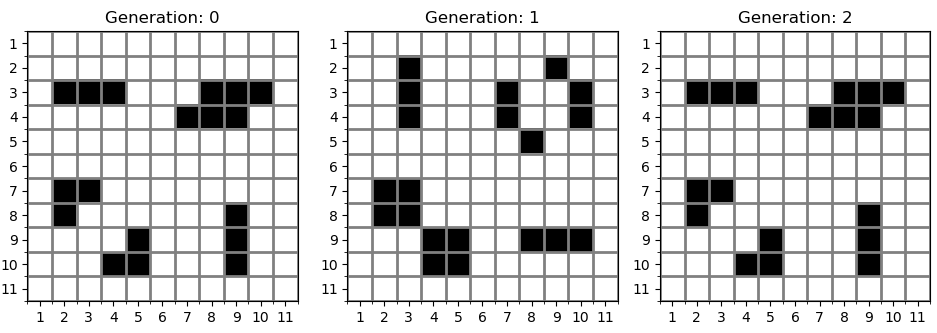
\includegraphics[width=\textwidth]{classic-vibrating.png}
  \caption{周而复始的图形}
  \label{fig:classic-vibrating}
\end{figure}

\section{氧气模型}

我们小组的目标是在细胞自动机的基础上模拟生态系统。氧气是模拟生态系统中的要素之一,本节将介绍我们小组定义的氧气模型。

\subsection{扩散规则}

在现实生活中,氧气可以在自由空间内扩散,最终平均扩散到空间各处,各处的氧气浓度一致。因此要模拟氧气,最重要的是模拟氧气随着时间的推移而扩散到自由空间内的性质。

我们使用迭代次数的增加表示时间的推移。棋盘上每个格子的体积一定,因此一个格子上所含有的氧气的量可以用氧气浓度的数值进行表示和参与运算。这里规定格子上氧气的浓度可以在某次迭代中超过1,但不能在连续的几次迭代中持续超过1。

对于一个格子而言,格子在下一轮氧气的浓度数值上等于格子在上一轮氧气浓度减去本轮扩散到其他格子的氧气浓度,再加上本轮其他格子扩散到当前格子的氧气浓度。

规定一个格子$c$在一轮扩散中氧气的总扩散量为上轮氧气浓度$last_c$的一半,对于与其相邻的包括它自身在内的9个格子$neighbor(c)$,每个格子$i$从$c$中获取的氧气的扩散量$shared_{c, i}$由以下公式进行计算:

\begin{equation}
  \label{equ:share-oxygen}
  shared_{c, i} = \frac{1}{2} \cdot last_c \cdot \frac{1 - min(1, last_i)}{\sum (1 - min(1, last_i))}, i \in neighbor(c)
\end{equation}

上述公式的物理意义是,在氧气扩散总量一定的前提下,格子在上一轮中氧气的浓度越小,在本轮中所分得的氧气浓度就越高。公式中分子和分母位置的$1 - min(1, last_i)$的含义是,氧气不向氧气浓度大于或等于1的格子扩散。

那么对于一个格子$c$,其本轮的氧气浓度由以下公式进行计算:

\begin{equation}
  \label{equ:gathering-oxygen}
  current_c = \frac{1}{2} \cdot last_c + shared_{i, c} , i \in neighbor(c)
\end{equation}

容易看出,按上面的公式\ref{equ:share-oxygen}和公式\ref{equ:gathering-oxygen}进行的计算是遵循物质守恒定律的。

对于棋盘边界上的格子,如果采用定值方法处理边界,则氧气浓度应该设置为1,且边界格子不参与氧气扩散量的计算。由公式\ref{equ:share-oxygen}知,边界格子亦不会吸收氧气。

如果采用镜像边界方法,则边界格子与非边界格子使用同样的规则进行迭代。

\subsection{氧气模型的实现}

我们在程序\underline{2.oxygen.py}中实现了上一小节中描述的氧气模型。

如图\ref{fig:oxygen-flow}所示的热力图中,蓝色表示氧气。格子中的氧气密度越高,格子上蓝色的程度就越深。后续章节中,我们使用绿色和红色分别表示生产者、消费者的种群密度,颜色越深,表示该格子上的种群密度越高。

如图\ref{fig:oxygen-flow},棋盘的初始状态随机给出,随后按照我们定义的氧气规则进行演化。

\begin{figure}[ht]
  \centering
  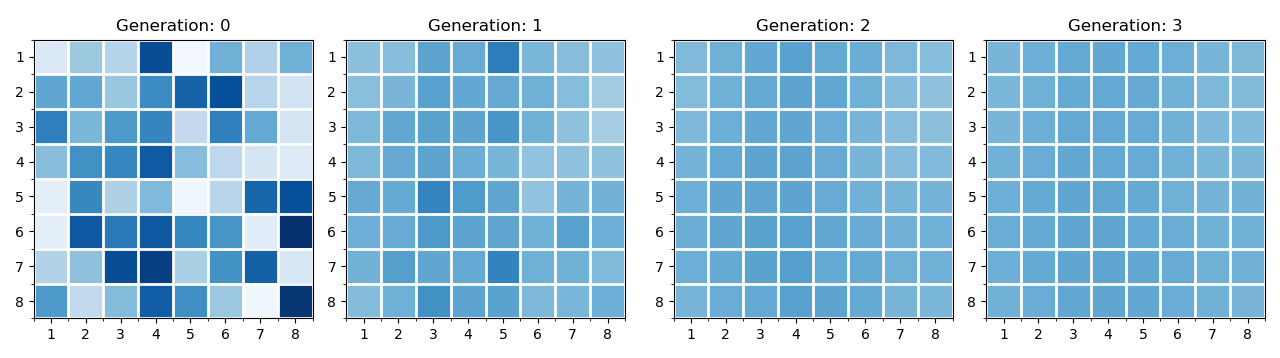
\includegraphics[width=\textwidth]{oxygen-flow.png}
  \caption{氧气在自由空间内的扩散}
  \label{fig:oxygen-flow}
\end{figure}

在图\ref{fig:oxygen-4polar-flow}和图\ref{fig:oxygen-polar-flow}中,我们还模拟了棋盘中氧气从一处或几处浓度峰值点向外自由扩散的情况。

\begin{figure}[ht]
  \centering
  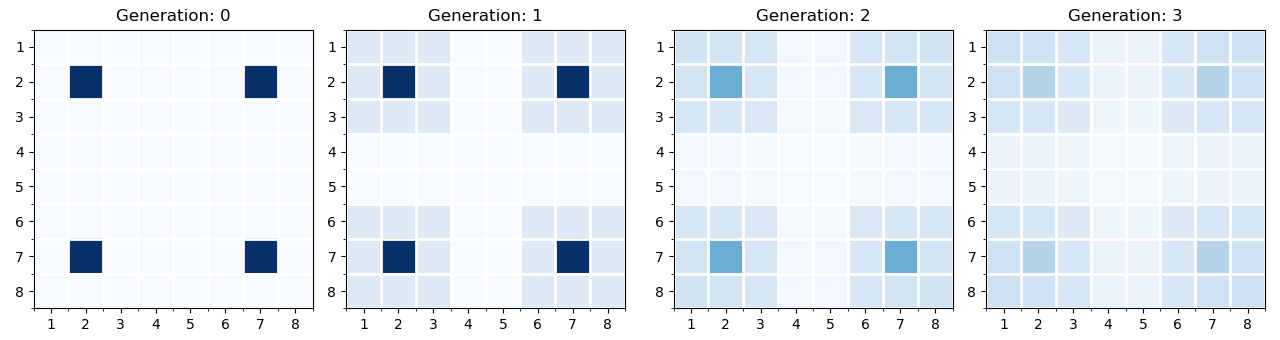
\includegraphics[width=\textwidth]{oxygen-4polar-flow.png}
  \caption{氧气从峰值点的扩散1}
  \label{fig:oxygen-4polar-flow}
\end{figure}

\begin{figure}[ht]
  \centering
  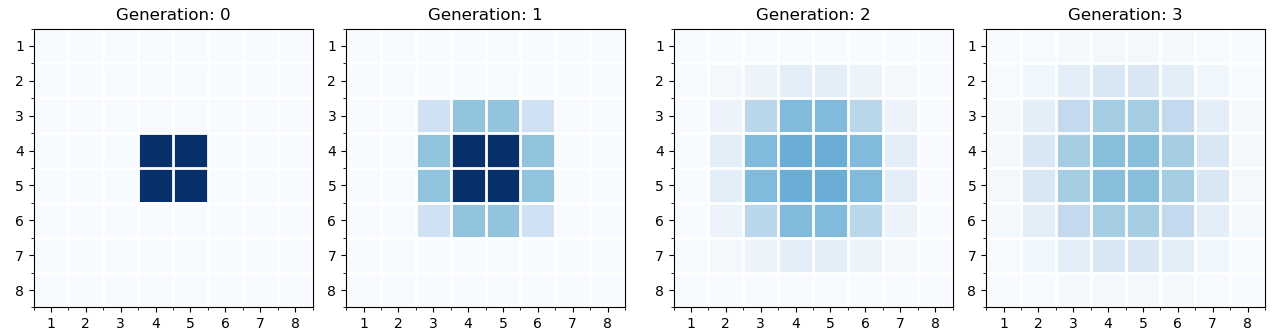
\includegraphics[width=\textwidth]{oxygen-polar-flow.png}
  \caption{氧气从峰值点的扩散2}
  \label{fig:oxygen-polar-flow}
\end{figure}

从图像上看,我们的氧气模型用较小的计算代价在一定程度上模拟了现实情形。

\section{生产者模型}

生态系统可分为生物部分和非生物部分。在上一节中,我们在非生物部分中选择了氧气要素进行了模拟;本节中,我们将模拟生物部分的基础——生产者。

\subsection{氧气生产规则}

生产者的基本功能是生产氧气。考虑生产者生产的氧气时,我们忽略生产者的呼吸作用,只考虑净光合作用的影响。

以下是光合作用的公式:

\begin{equation}
  12H_2O + 6CO_2 \overset{sun}{\rightarrow} C_6H_{12}O_6 + 6O_2 + 6H_2O
  \label{equ:photosynthesis}
\end{equation}

从光合作用的公式来看,光合作用的原料是水和二氧化碳,条件是阳光,最终产物是葡萄糖、水和氧气。我们模拟的生态系统中,缺少对水和二氧化碳的模拟。而我们将光照强度$sunLevel$作为影响生产者生产氧气速率的因素,其取值范围在$[0, 1]$上。光合作用的最终产物之一葡萄糖的贡献体现在下一小节中生产者种群密度的增长上。

与氧气浓度类似,我们定义单位格子上生产者的数量为种群密度$producerDensity$,其取值范围在$[0, 1]$上。生产者的种群密度也是其生产氧气速率的影响因素之一。定义种群密度的临界值为0.01,若低于0.01,则认为当前格子上的生产者种群密度过低,不足以继续发展而消亡。

我们用迭代表示时间的推移,定义一个格子上的生产者每次迭代产生的氧气$producedOxygen$(在数值上表现为氧气浓度的增量)按以下公式计算:

\begin{equation}
  producedOxygen = sunLevel \cdot producerDensity \cdot max(1 - oxygenLevel, 0)
\end{equation}

公式中$oxygenLevel$为生产者所在格子的氧气浓度。公式的生物学含义是,在其他条件一定的前提下,氧气浓度越高(意味着二氧化碳的浓度越低),生产者产生氧气的能力就越受到限制。此公式也保证了生产者生产氧气后,其所在格子的氧气浓度不会因此而超过1。

图\ref{fig:producer-produce}为程序\underline{3.producer.no-growth.py}模拟的生产者生产氧气的过程。程序先给出随机氧气分布然后开始迭代,氧气从生产者处产生,尔后扩散到环境中的其他部分(体现为棋盘上蓝色加深)。

\begin{figure}[ht]
  \centering
  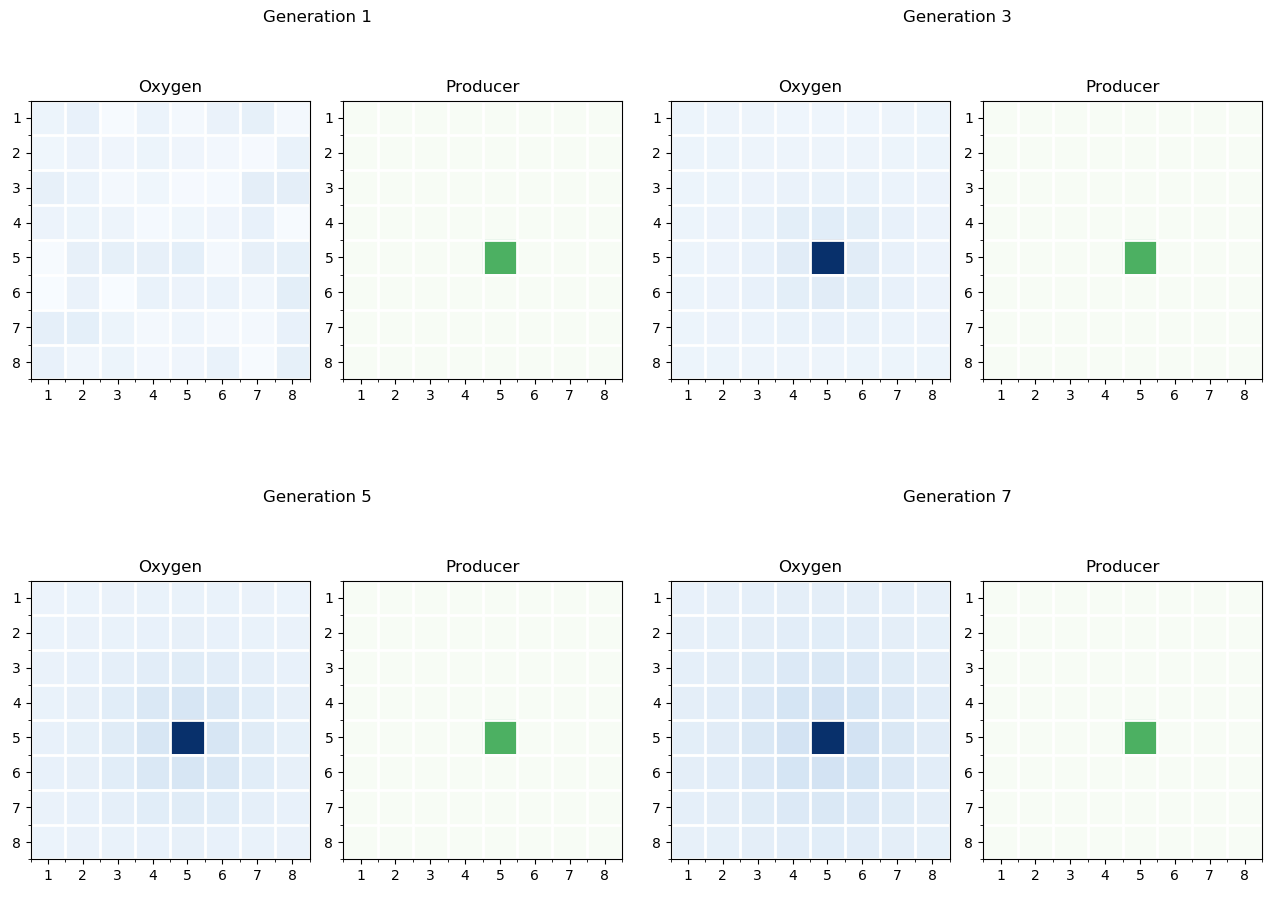
\includegraphics[width=\textwidth]{producer-produce.png}
  \caption{生产者生产氧气}
  \label{fig:producer-produce}
\end{figure}

\subsection{种群密度的增长规则} \label{sec:density-growth-curve}

从生物学的角度上看,生物种群密度的增长随时间的推移而呈现出S型曲线,即种群的增长率一直下降,增长速率先增加后下降。

\begin{figure}[ht]
  \centering
  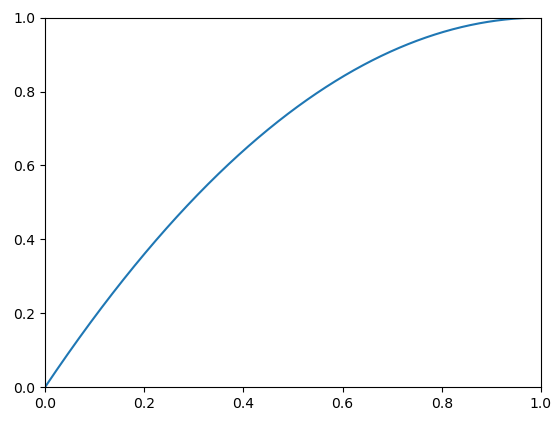
\includegraphics[scale=0.6]{density-curve.png}
  \caption{理想种群密度曲线}
  \label{fig:density-curve}
\end{figure}

我们定义\textbf{理想种群密度曲线$dt(x)$}为二次曲线$y = -(x-1)^2 + 1$。如图\ref{fig:density-curve}所示,横轴为上次迭代中生产者的种群密度,纵轴为本次迭代生产者的种群密度。整条曲线在直线$y=x$上方,表示种群密度保持增长;且曲线斜率不断下降,表示种群增长率不断下降。

\begin{equation}
  dt:= density_{current} = -(density_{last} - 1)^{2} + 1
  \label{equ:density-curve}
\end{equation}

为了体现光照强度对生产者生产的影响,在一次迭代中,生产者的实际种群密度使用下面的公式进行修正:

\begin{equation}
  density_{current} = density_{last} + (dt(density_{last}) - density_{last})) \cdot sunLevel
\end{equation}

\subsection{繁衍规则}

类似于康威生命游戏中细胞的增殖,我们模拟生态系统中的生产者按以下规则在新的格子上产生种群:设当前格子生产者的种群密度为$density$,则在其不包括自身的8个邻居中,对于每个邻居格子,若此邻居格子上没有生产者,则有$\frac{density}{8}$的概率在这个格子上产生种群密度为0.02的生产者。

按上述规则进行迭代,当前格子上生产者的种群密度越高,就越容易将种子传播到邻居格子处,播种出新的群落,这是符合常识的。

程序\underline{3.producer.py}模拟了生产者增长和繁衍的过程,其结果如图\ref{fig:producer-growth}所示。

\begin{figure}[ht]
  \centering
  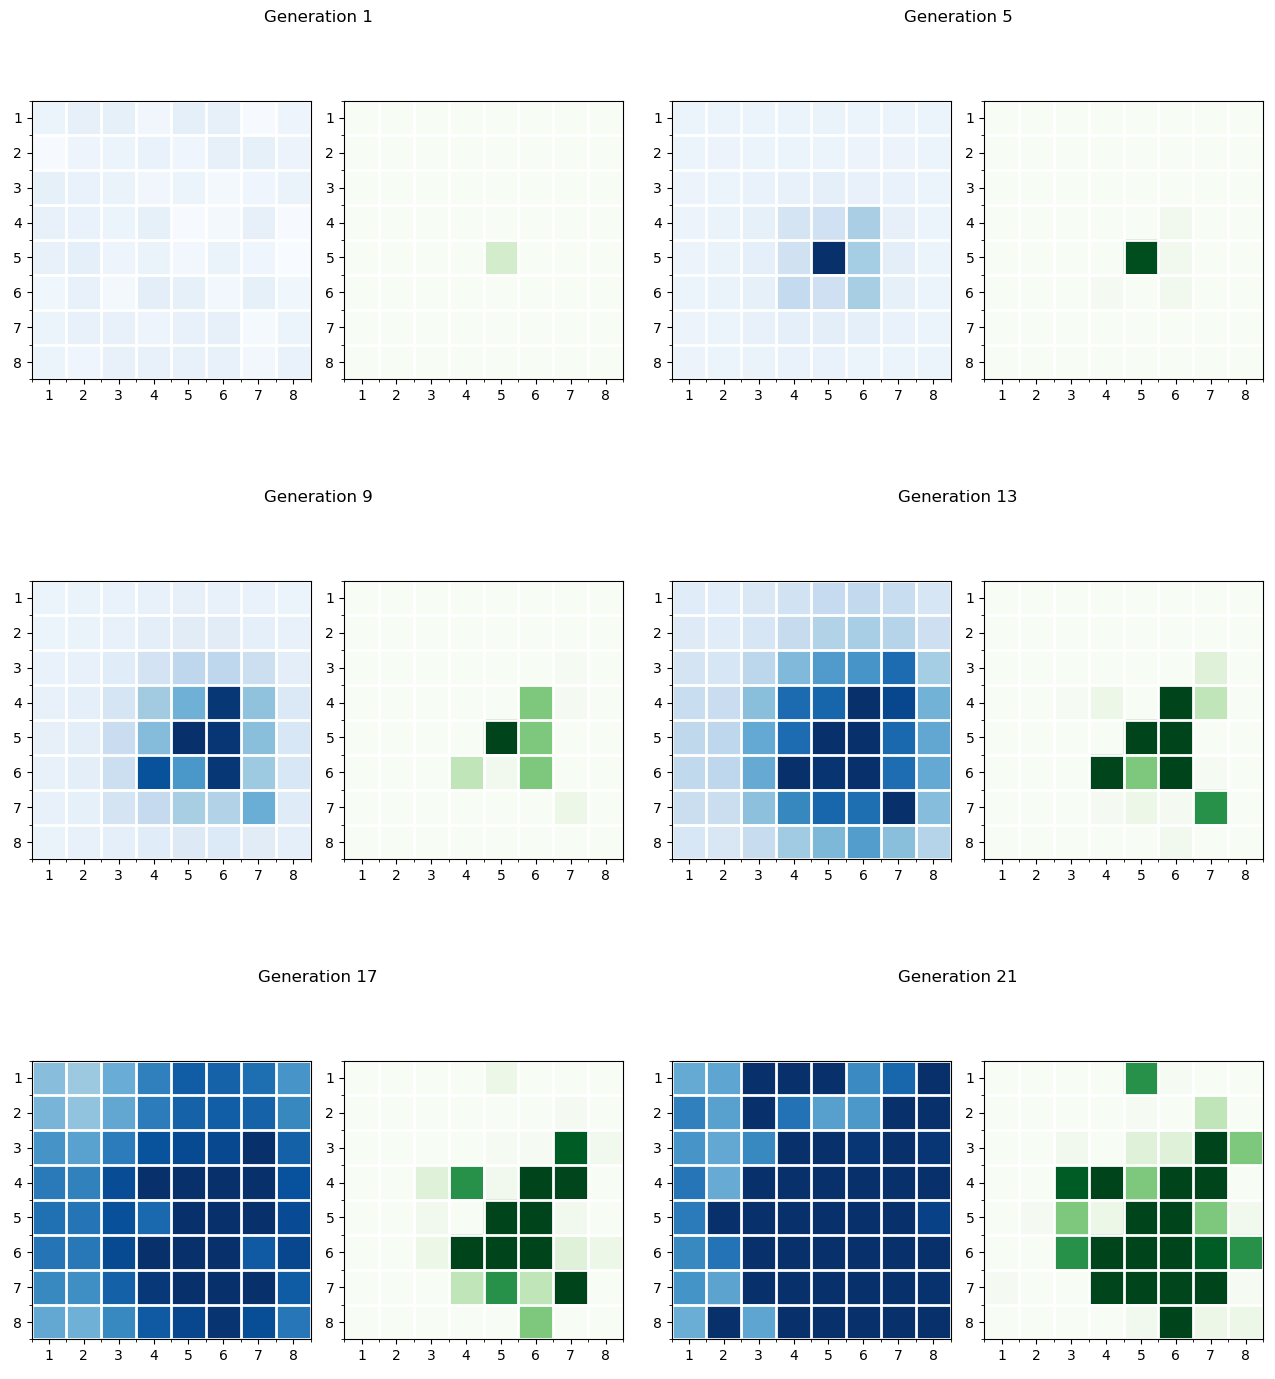
\includegraphics[width=\textwidth]{producer-growth.png}
  \caption{生产者的增长和繁衍}
  \label{fig:producer-growth}
\end{figure}

\section{消费者模型}

消费者是生态系统的生物部分的另一个重要的角色;本节将介绍我们小组设计的消费者模型。

\subsection{呼吸、捕食和种群增长} \label{sec:consumer-growth-rule}

消费者不能自己进行光合作用,需要消耗氧气进行呼吸和食用生产者作为能量来源。呼吸作用是光合作用(公式\ref{equ:photosynthesis})的逆过程,从光合作用的公式来看,单位消费者需要消耗0.5单位的氧气和0.5单位的生产者来保证自身种群的增长。当氧气和生产者能够满足消费者的需求时,消费者也按照\ref{sec:density-growth-curve}小节中的种群密度曲线进行增长。定义消费者呼吸、捕食和种群增长的规则如下:

设当前格子消费者的种群密度为$density$,则当前格子上的消费者需氧量$needOxygen$(以氧气浓度计算)为$\frac {1}{2} \cdot density$,需要的食物量$needFood$(以生产者种群密度计算)为$\frac {1}{2} \cdot density$。

\begin{enumerate}
  \item 计算当前格子上当前种群密度的消费者的需氧量$need$。若当前格子上实际含氧量$actual$小于$need$,则消费者的种群密度下降为$density \cdot \frac{need - actual}{need}$,并消耗$actual$量的氧气;否则消耗$need$量的氧气。
  \item 计算当前格子上当前种群密度的消费者的食物需求量$need$(若第一步计算中消费者的种群密度下降了,则使用下降后的种群密度计算$need$)。若当前格子上的生产者种群密度$actual$小于$need$,则生产者的种群密度下降为$density \cdot (\frac{1}{2} + \frac{1}{2} \cdot \frac{need - actual}{need})$,并消耗$actual$量的生产者;否则消耗$need$量的生产者。
  \item 若经过前两步计算后,消费者消耗了$need$量的氧气和生产者,则表示环境适宜,消费者按照理想种群密度曲线进行增长(公式\ref{equ:density-curve})。
\end{enumerate}

在我们设计的消费者规则中,氧气浓度比食物更重要些,缺乏氧气比缺乏食物更难存活。这是考虑到日常生活的经验中,生物缺少氧气会导致窒息死亡,但在食物短缺的情况下往往还能依据自身储备的碳量存活一段时间。

\subsection{移动规则}

消费者显著区别于生产者之处为,消费者可以进行移动,以寻找氧气和食物而不是坐以待毙。

消费者在移动时,将自己的8个邻居格子中本轮迭代和上轮迭代中没有其他消费者占据的邻居格子加入候选列表。若候选列表为空,则本轮不进行移动。若候选列表不为空,则按公式\ref{equ:cell-score}逐个计算候选列表中格子的分数,然后选择得分最高的格子移动。

\begin{equation}
  \label{equ:cell-score}
  score = oxygenLevel \cdot weight_{oxygen} + producerLevel \cdot weight{producer}
\end{equation}

公式\ref{equ:cell-score}中,$oxygenLevel$和$producerLevel$分别为对应格子的氧气浓度和生产者种群密度。$weight$为权重。我们小组的程序中,氧气权重和生产者种群密度权重分别取值0.6和0.4。

程序\underline{4.consumer.no-emerge.py}模拟了消费者的呼吸、捕食和种群增长和移动过程,其结果如图\ref{fig:consumer-move}所示。

\begin{figure}[ht]
  \centering
  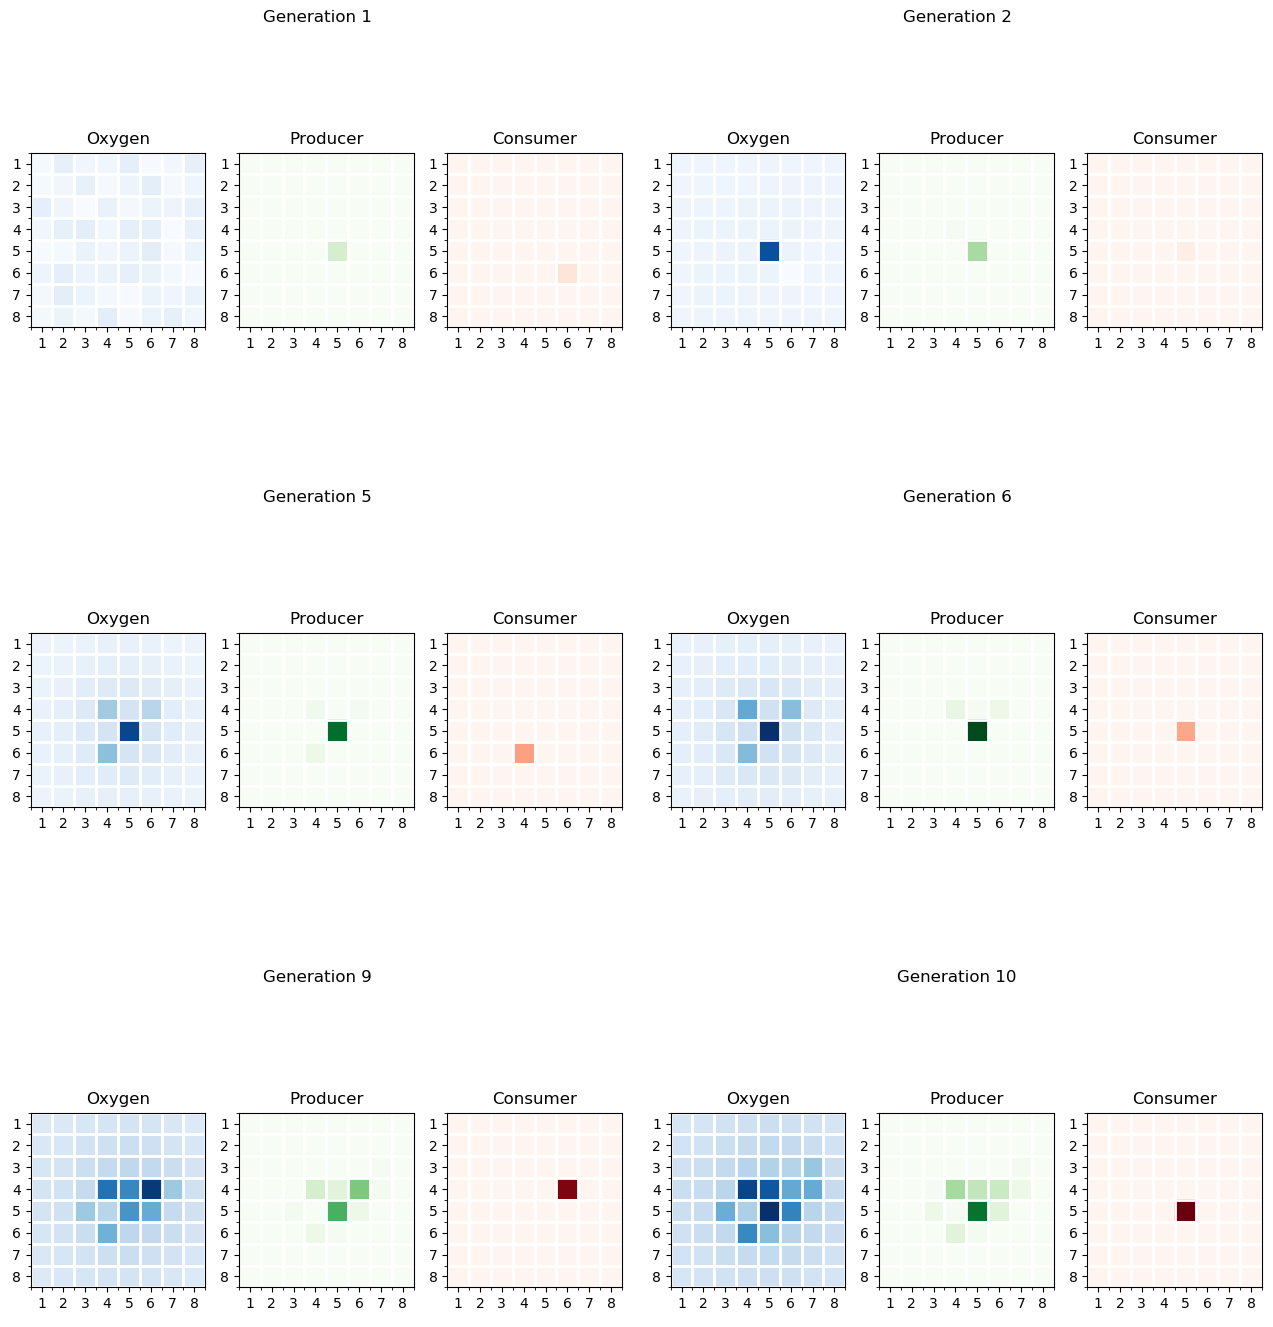
\includegraphics[width=\textwidth]{consumer-move.png}
  \caption{消费者的呼吸、捕食和种群增长和移动}
  \label{fig:consumer-move}
\end{figure}

\subsection{繁衍规则}

消费者也类似于生产者,具有繁衍种群的特性。设当前格子消费者的种群密度为$density$,则在其不包括自身的8个邻居中,对于每个邻居格子,若此邻居格子上没有消费者,则有$\frac{density}{8}$的概率在这个格子上产生种群密度为0.02的消费者。

程序\underline{4.consumer.py}模拟了完整的消费者模型,模拟结果如图\ref{fig:consumer}所示。

\begin{figure}[ht]
  \centering
  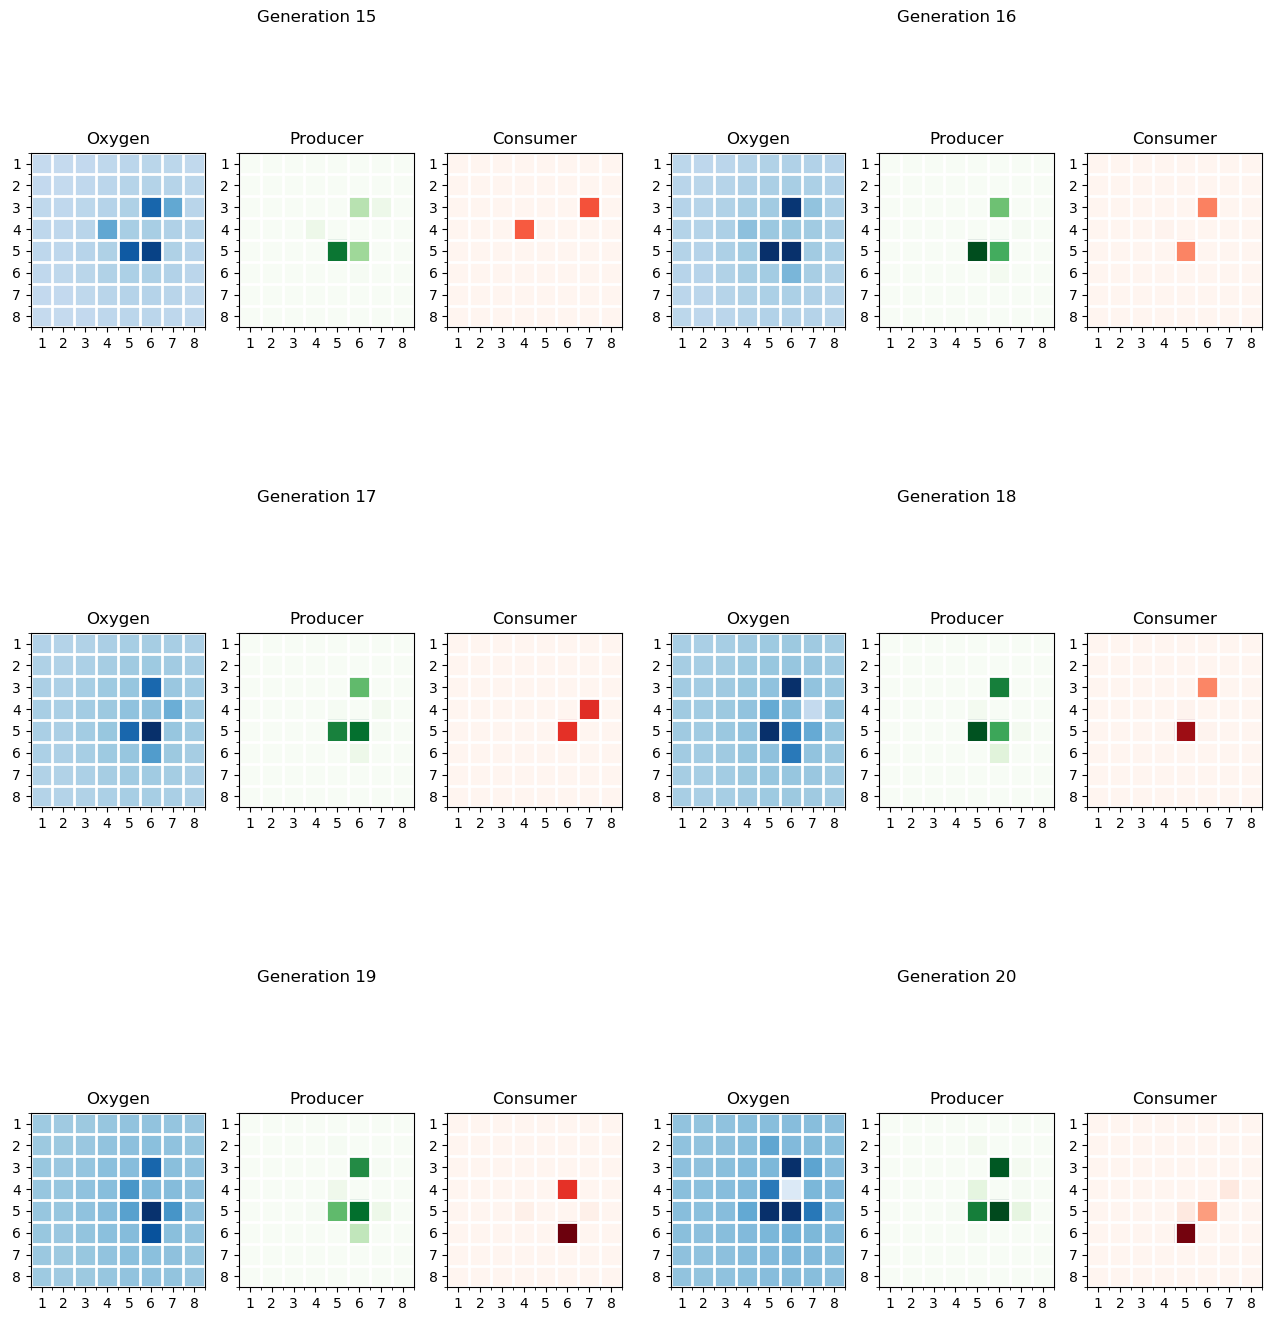
\includegraphics[width=\textwidth]{consumer.png}
  \caption{具有完整行为的消费者}
  \label{fig:consumer}
\end{figure}

\section{模拟生态系统}

通过建立氧气模型、生产者模型和消费者模型,我们已经取得了模拟一个简单的生态系统所需要的全部积木。将这三片积木拼装在到一个棋盘中(或者说是在z轴方向层叠的三块棋盘上),即可模拟出一个简单的生态系统。为了平衡氧气的产生速率与生产者、消费者的活动速率,程序中计算迭代的顺序为:氧气迭代4次,生产者和消费者各迭代1次。在程序\underline{5.ecosystem.py}模拟了完整的生态系统。

\begin{figure}[ht]
  \centering
  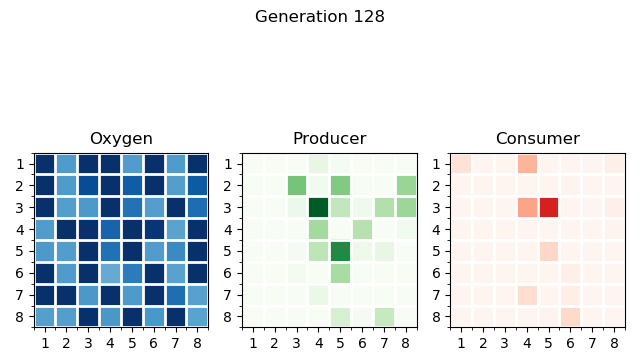
\includegraphics[scale=0.75]{weak-light.png}
  \caption{弱光照条件(0.2)下迭代128次后的生态系统}
  \label{fig:weak-light}
\end{figure}

\begin{figure}[ht]
  \centering
  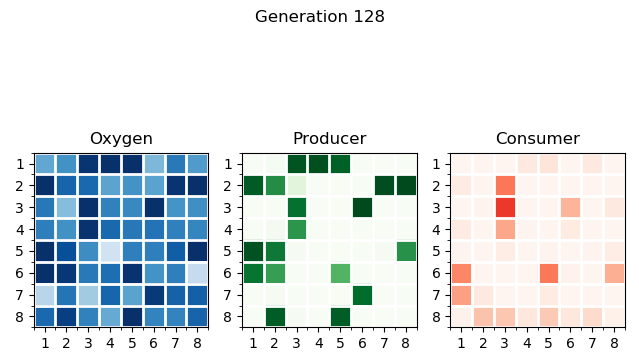
\includegraphics[scale=0.75]{medium-light.png}
  \caption{中等光照条件(0.5)下迭代128次后的生态系统}
  \label{fig:medium-light}
\end{figure}

\begin{figure}[ht]
  \centering
  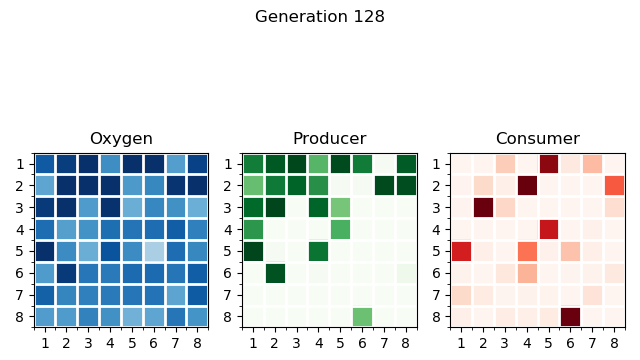
\includegraphics[scale=0.75]{abundant-light.png}
  \caption{强光照条件(0.8)下迭代128次后的生态系统}
  \label{fig:abundant-light}
\end{figure}

利用该程序,并控制光照强度变量,我们获得了在三种不同强度的光照条件下模拟生态系统迭代128次后的图形,如图\ref{fig:weak-light}、图\ref{fig:medium-light}和图\ref{fig:abundant-light}所示。从图中可以很明显地看出不同光照条件下生态系统的差异。生态系统的光照条件越充足,所能承载的消费者种群密度就越高。

图\ref{fig:ecosystem}为一个模拟生态系统的演化过程。

\begin{figure}[ht]
  \centering
  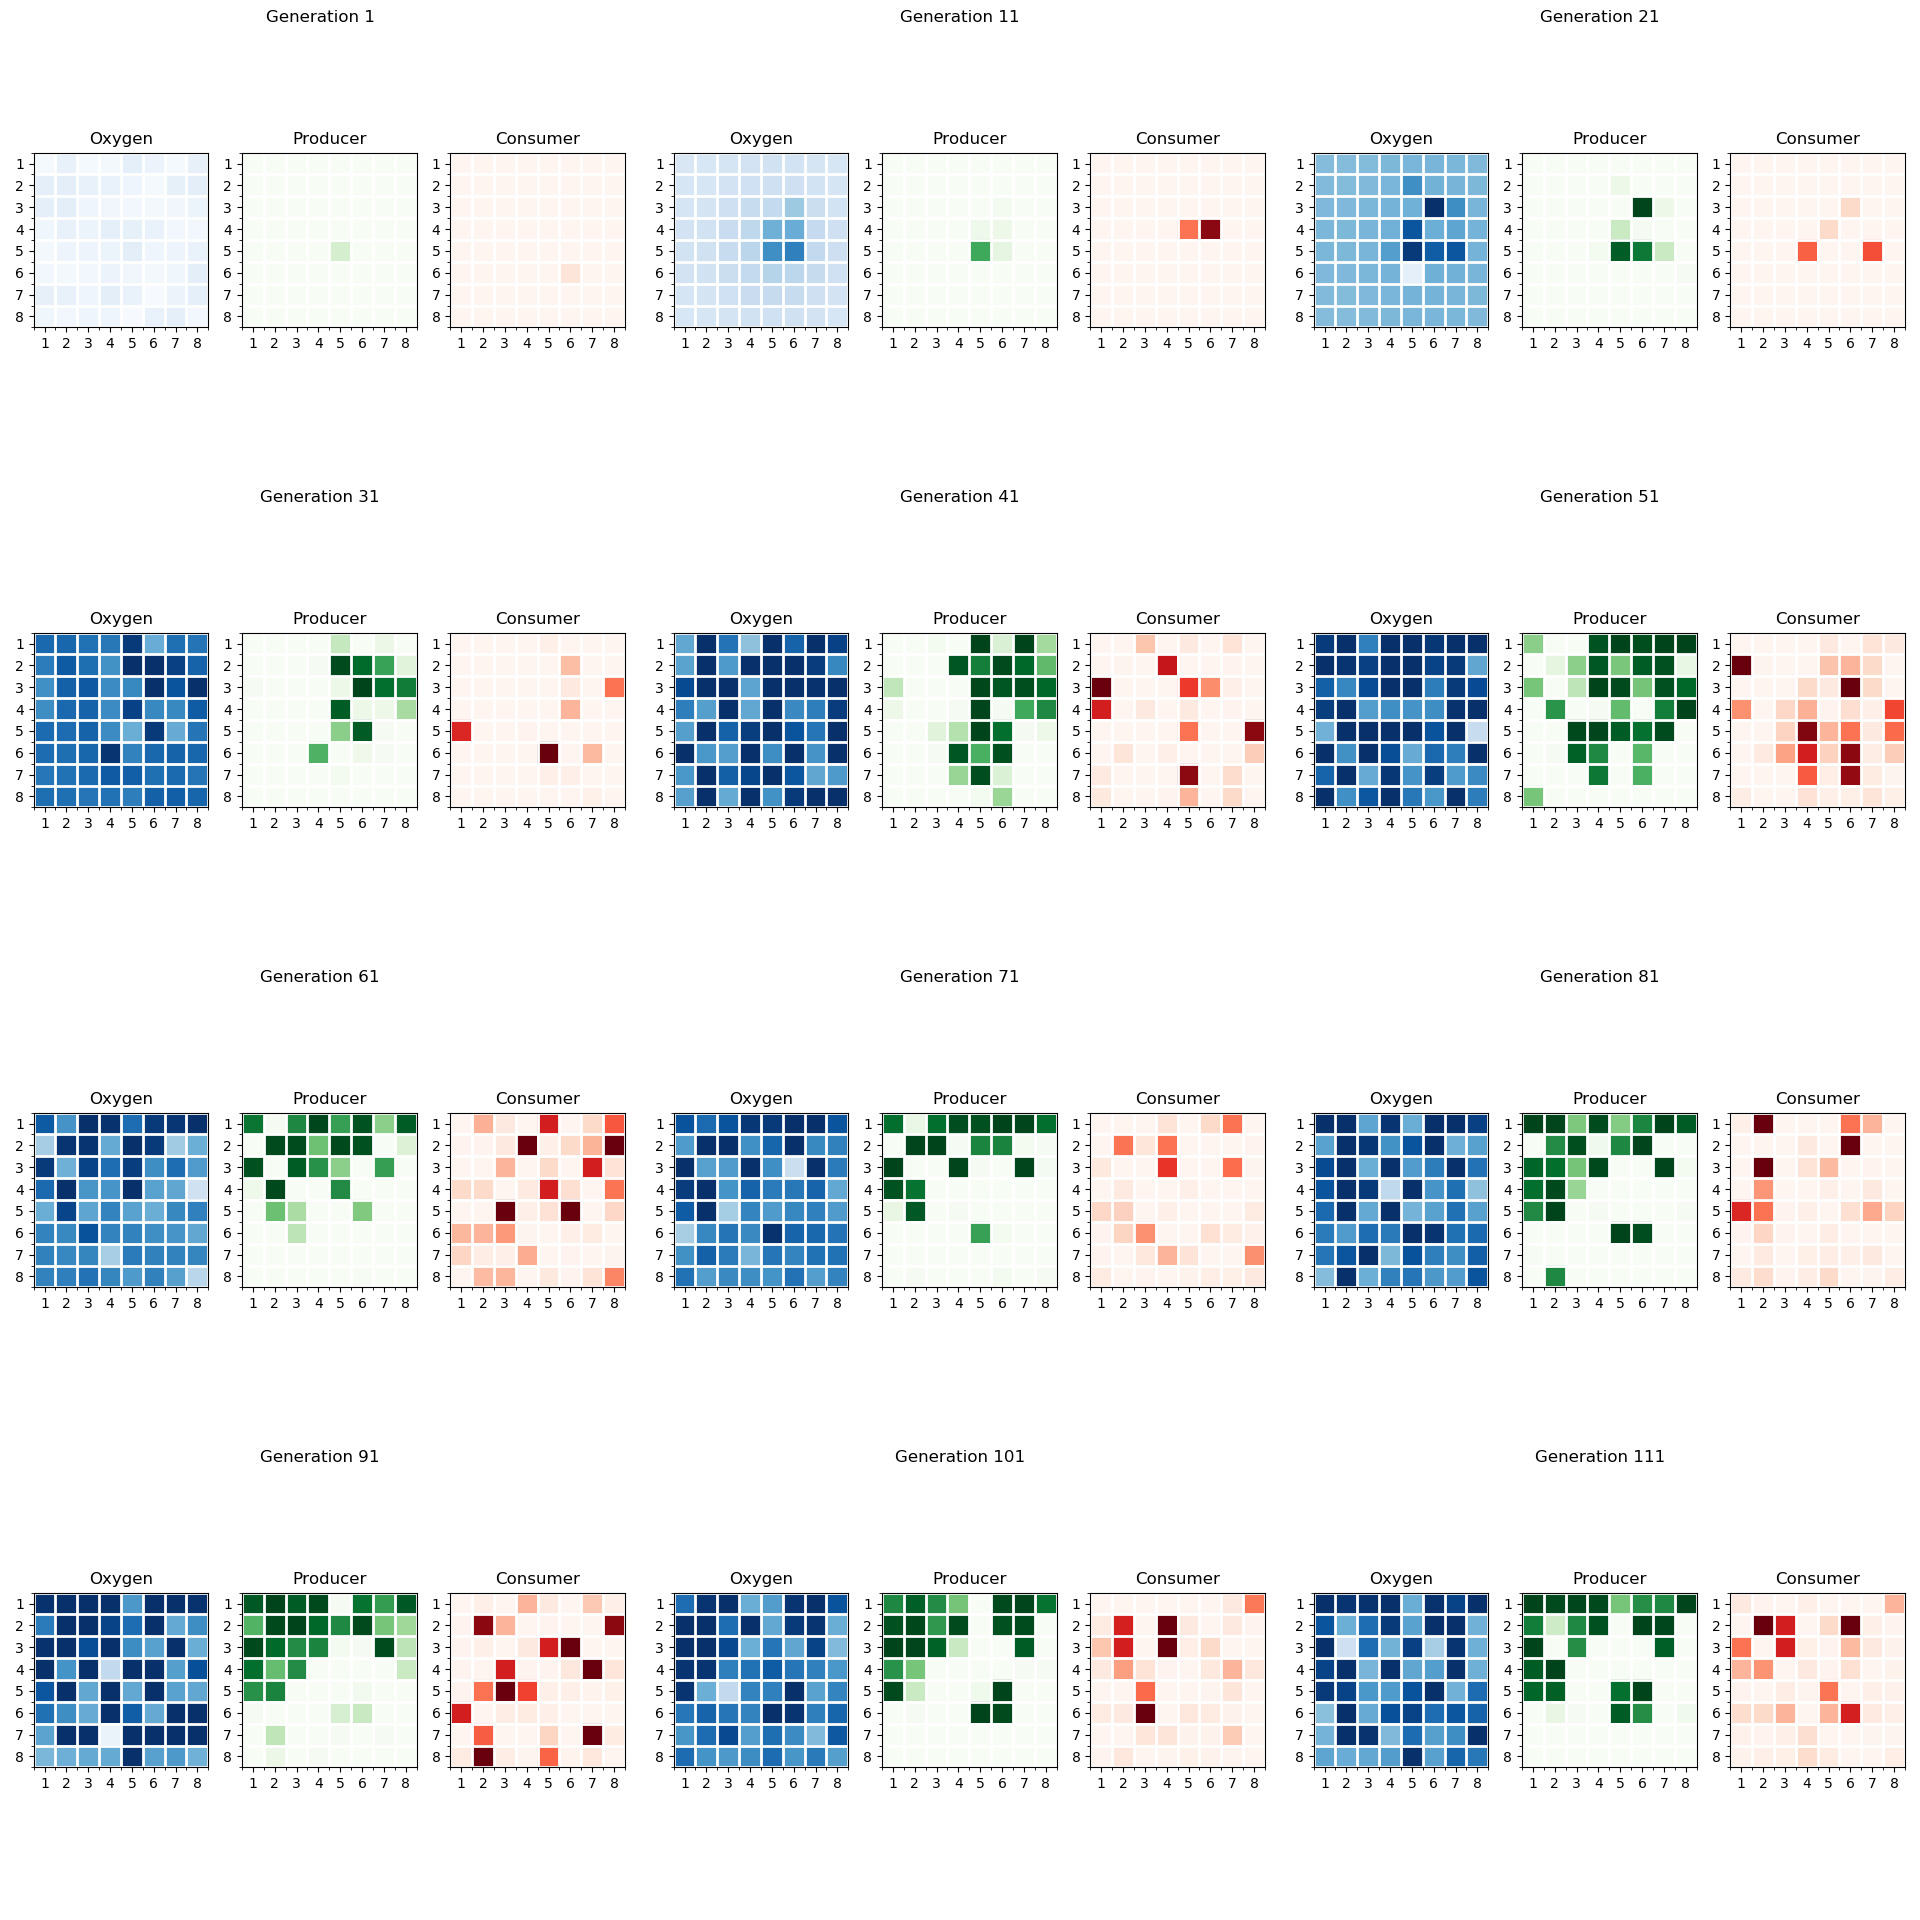
\includegraphics[width=\textwidth]{ecosystem.png}
  \caption{一个生态系统的演化过程}
  \label{fig:ecosystem}
\end{figure}

\section{结语}

我们小组提出的关于生态系统的计算模型,从一定程度上模拟了现实世界中的生态系统。

我们也认识到提出的模型中存在有待商榷之处。例如,在基础的氧气模型中,我们规定单位格点的氧气密度不能超过1,我们也尝试建立数学规则将氧气密度约束在$[0, 1]$上。但在实际的实验数据中,总会有些意料之外的情形。这说明我们提出的氧气模型是存在一定的缺陷的。

我们在对细胞自动机进行“拓展”的时,其实已经破坏了细胞自动机的一些性质。举一例说,消费者的移动规则破坏了细胞自动机的平行计算性。因为在计算移动时,不仅使用了上一轮的数据,还使用了本轮的数据,因此遍历元胞的先后顺序会影响计算的结果。综上所述,或许不能称我们得到的模型为“细胞自动机”。

这篇报告所体现的内容并不是我们最初想法的全部。报告原题为《使用细胞自动机和遗传算法模拟简单生态系统》,原本设想是在建立氧气、生产者和消费者模型的基础上,结合遗传算法,模拟在不同的环境参数下,自然选择和生物进化的过程。但编程过程中出现了一些问题。时间不足,只好作罢。希望日后有机会继续完善这个模型。

\end{document}
